\section{E-Mail Security}
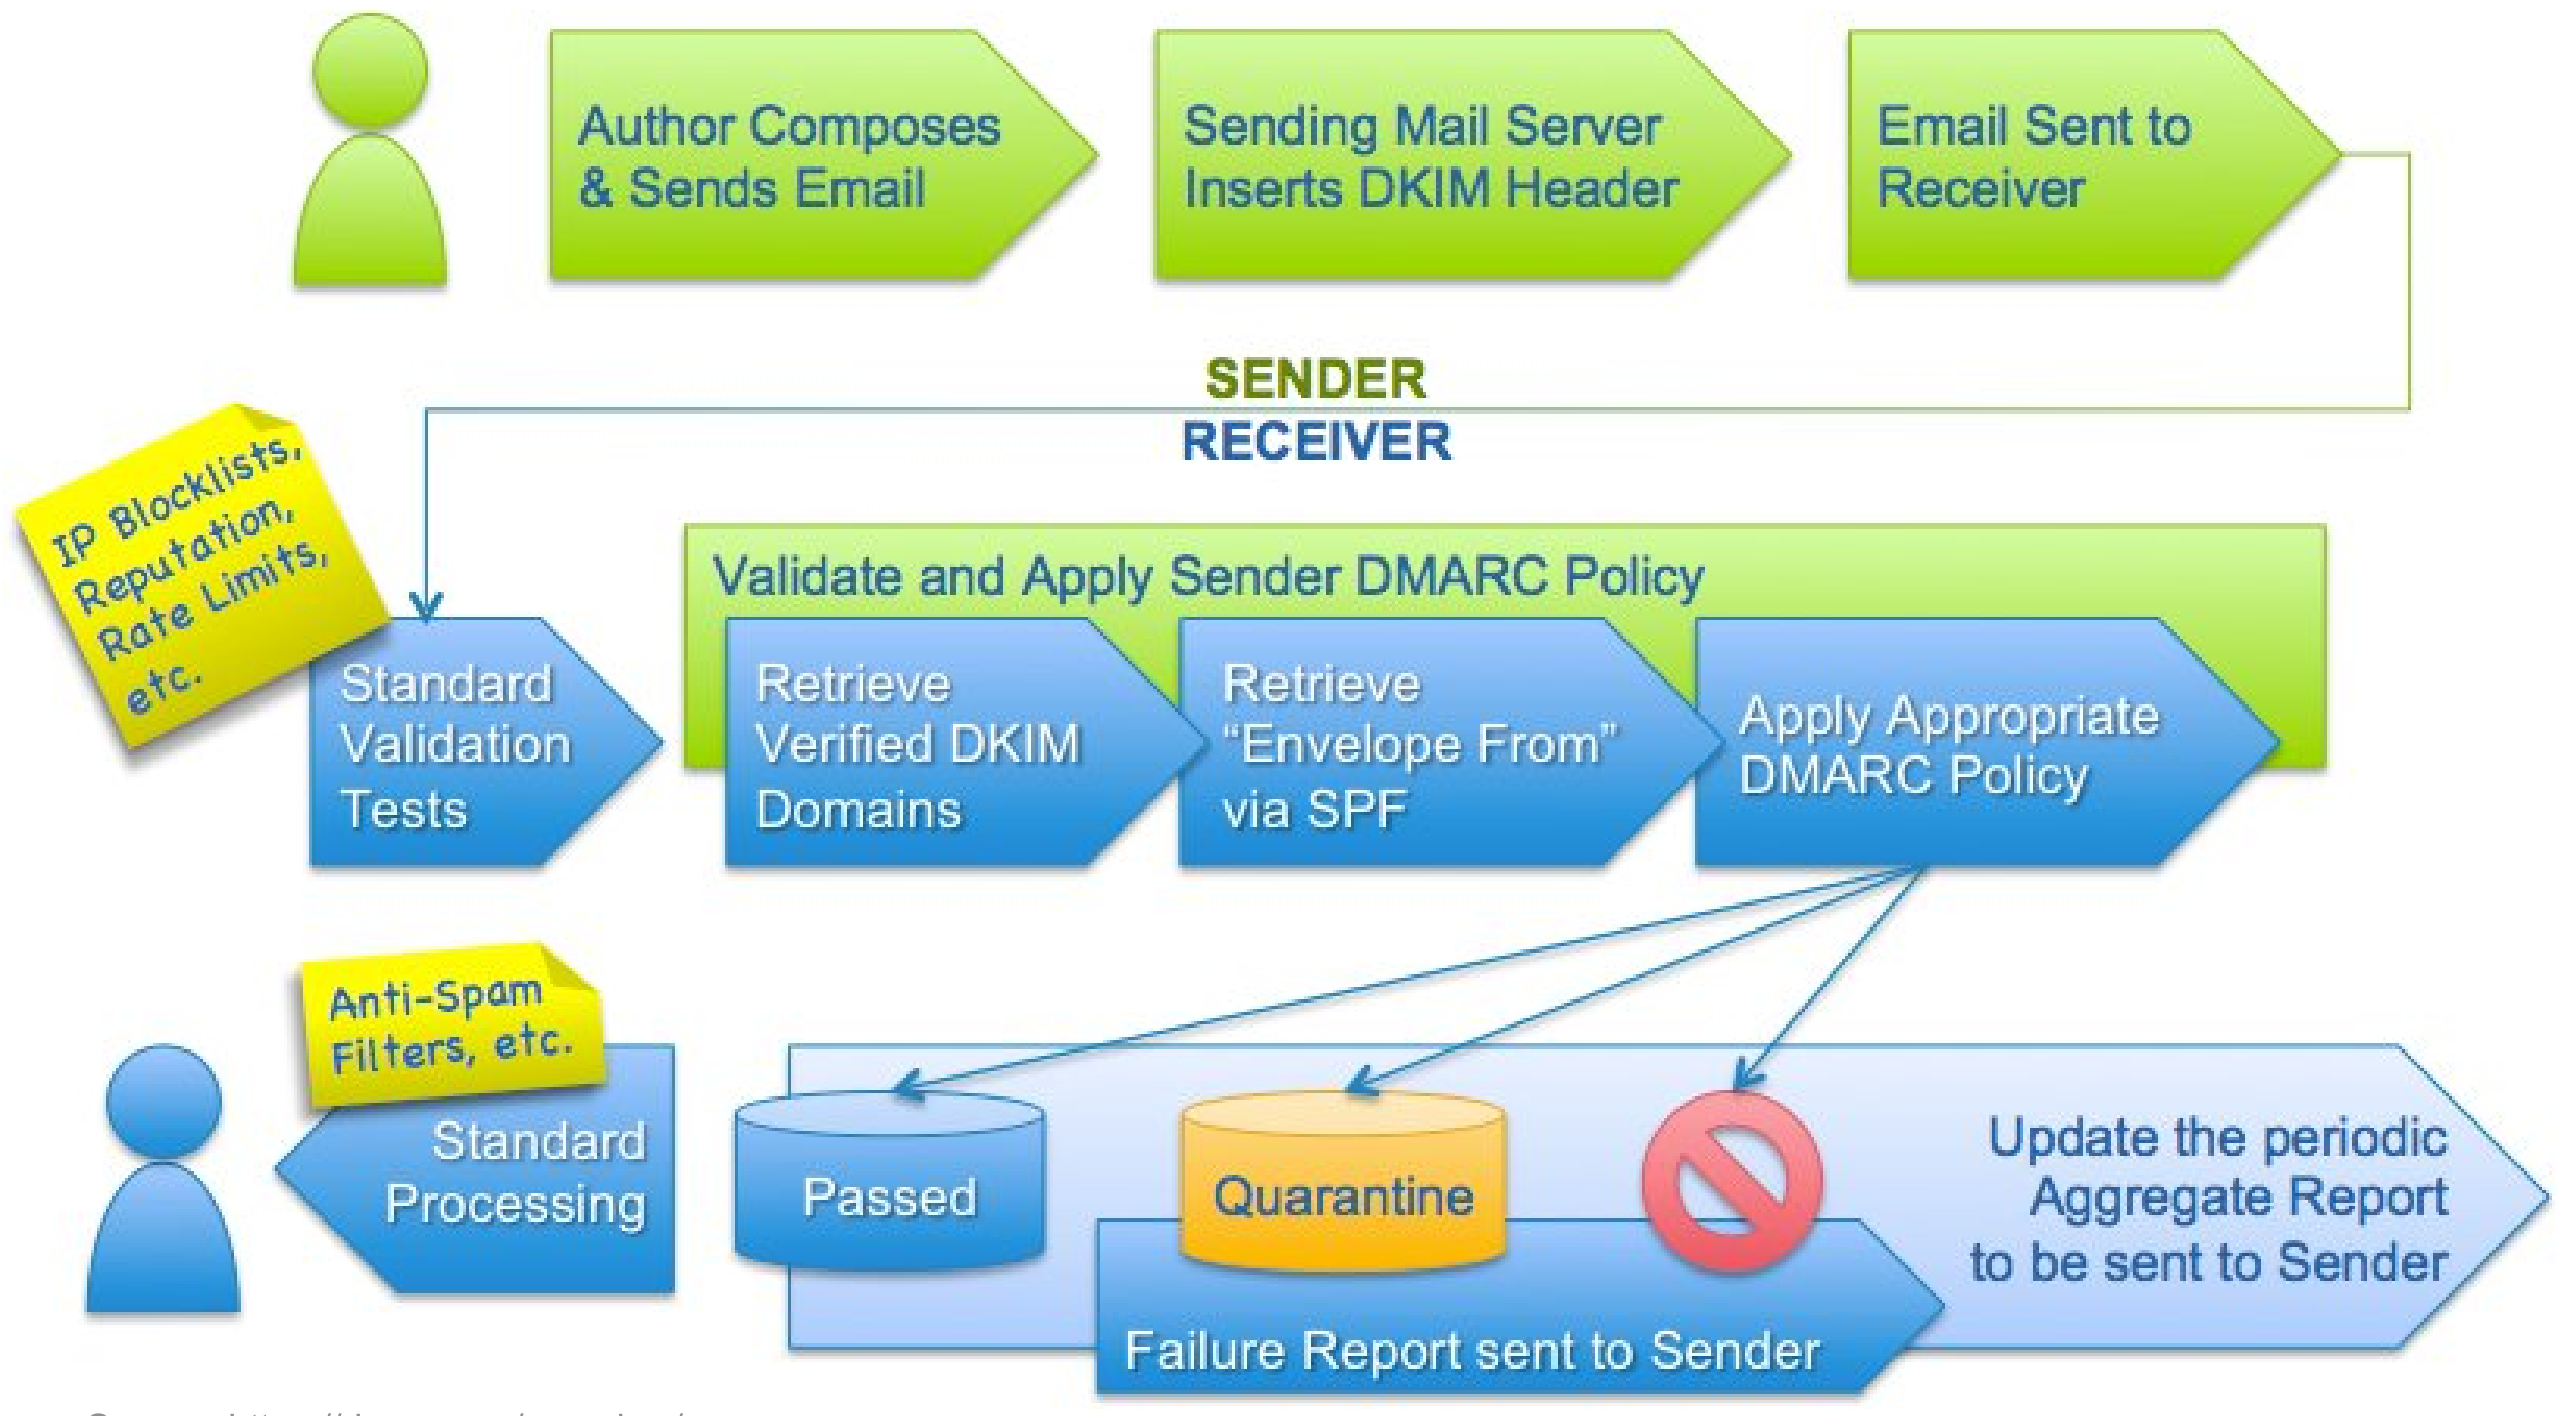
\includegraphics[width=\linewidth]{email-security.png}



\subsection{SPF (Sender Policy Framework)}
SPF allows senders to define which IP addresses are allowed to send mail for a particular domain. SPF alone is limited to detecting a forged sender claim in the envelope of the email, which is used when the mail gets bounced.
Only in combination with DMARC can it be used to detect the forging of the visible sender in emails, a technique often used in phishing and email spam.\\

SPF-Records are TXT DNS-Records. Used Codes in TXT content:
\begin{itemize}
  \item \textbf{v}: Version of record. E.g.: v=SPF1
  \item \textbf{ip4}: Allowed IP addresses.
  \item \textbf{-all}: All other listed senders are not authorized.
  \item \textbf{include}: More SPF-Records which should be checked.
\end{itemize}

\subsubsection{Check via console}
An SPF check can be made via console:
\begin{lstlisting}
  dig -t txt compass-security.com +noall +answer
  compass-security.com    70    IN    TXT     "v=spf1 mx ipv4:193.135.215.47/32"
  compass-security.com    70    IN    TXT     "MS=ms81325037"

  #With short param:
  dig +short  compass-security.com txt
  "v=spf1 mx ipv4:193.135.215.47/32"
\end{lstlisting}

\subsubsection{Where to check in metadata}
\paragraph{Passed}
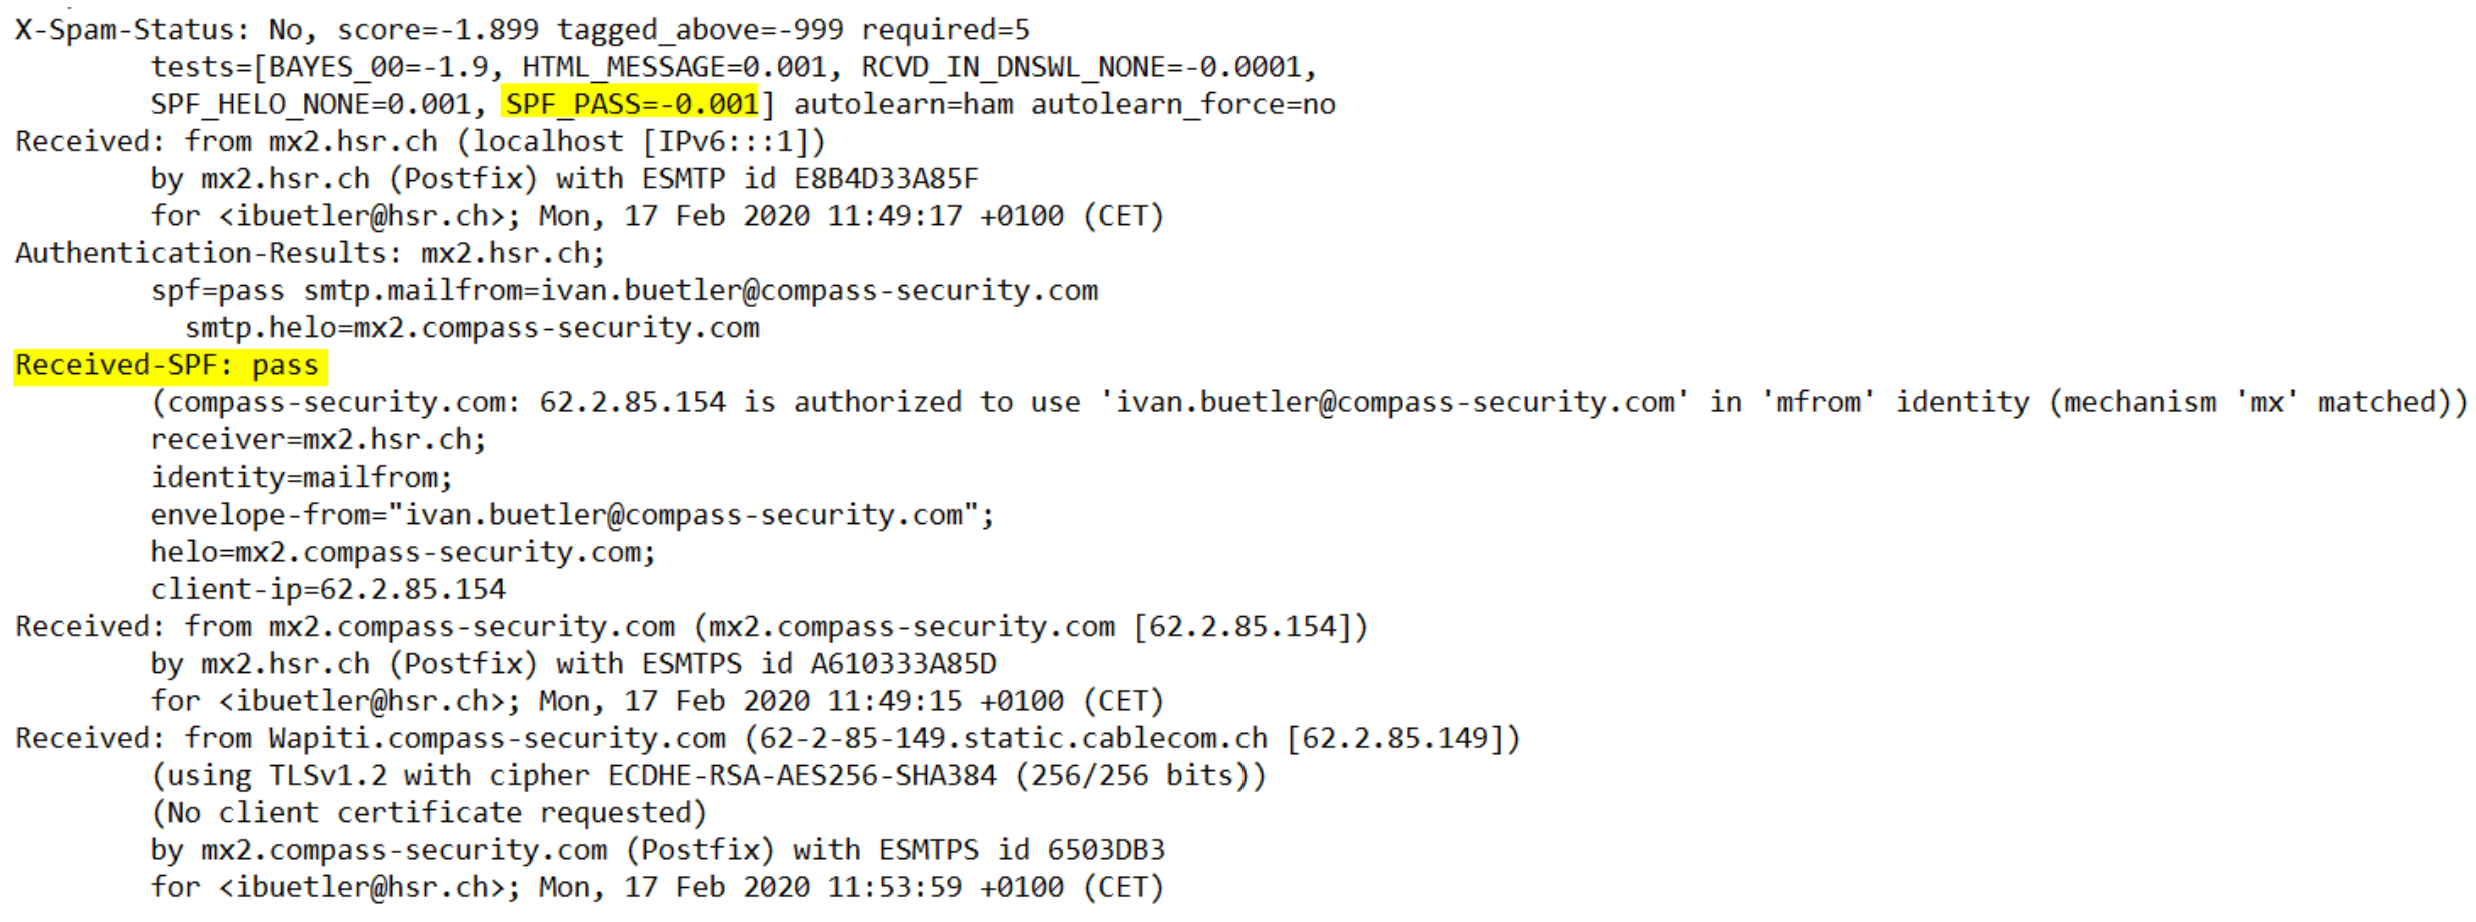
\includegraphics[width=\linewidth]{spf-check-yes.png}\\
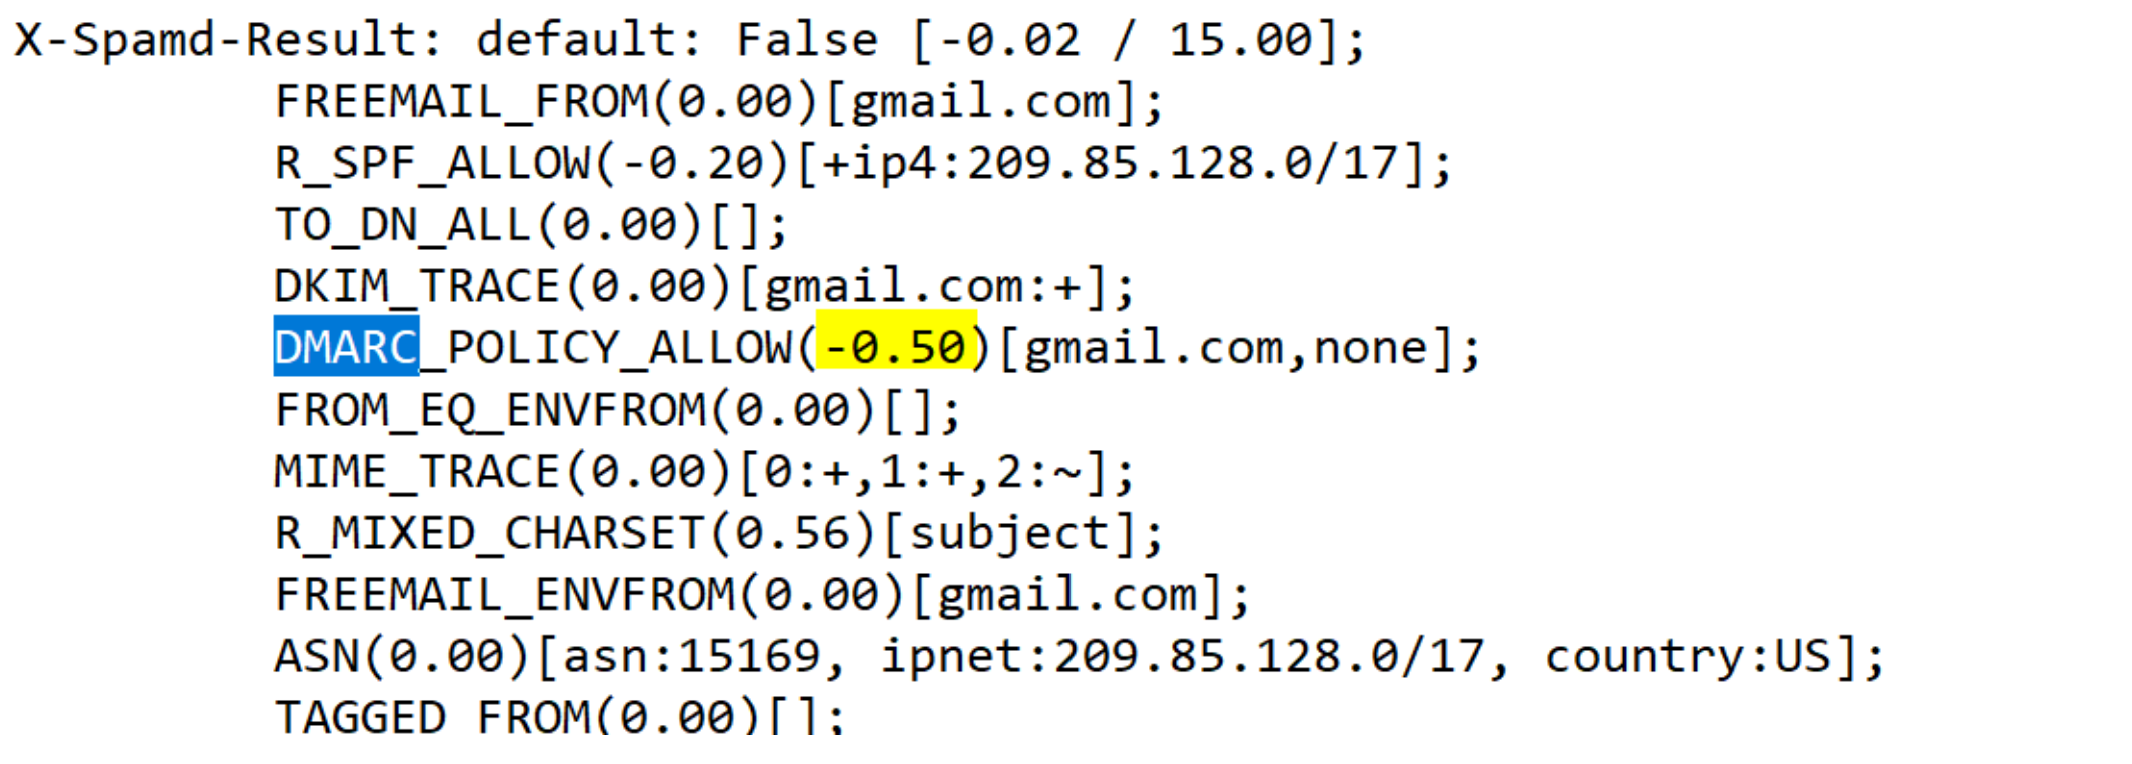
\includegraphics[width=\linewidth]{spf-check-yes-2.png}

\subsubsection{Bypass SPF}
Have a legit email address which passes the check in the header in the E-Mail envelope and the spoofed email address in the email header.





\subsection{DKIM (Domain Keys Identified Mail)}
DKIM provides an encryption key and digital signature that verifies that an email message was not faked or altered.
It uses ``public key cryptography'' to verify that an email message was sent from an authorized mail server.
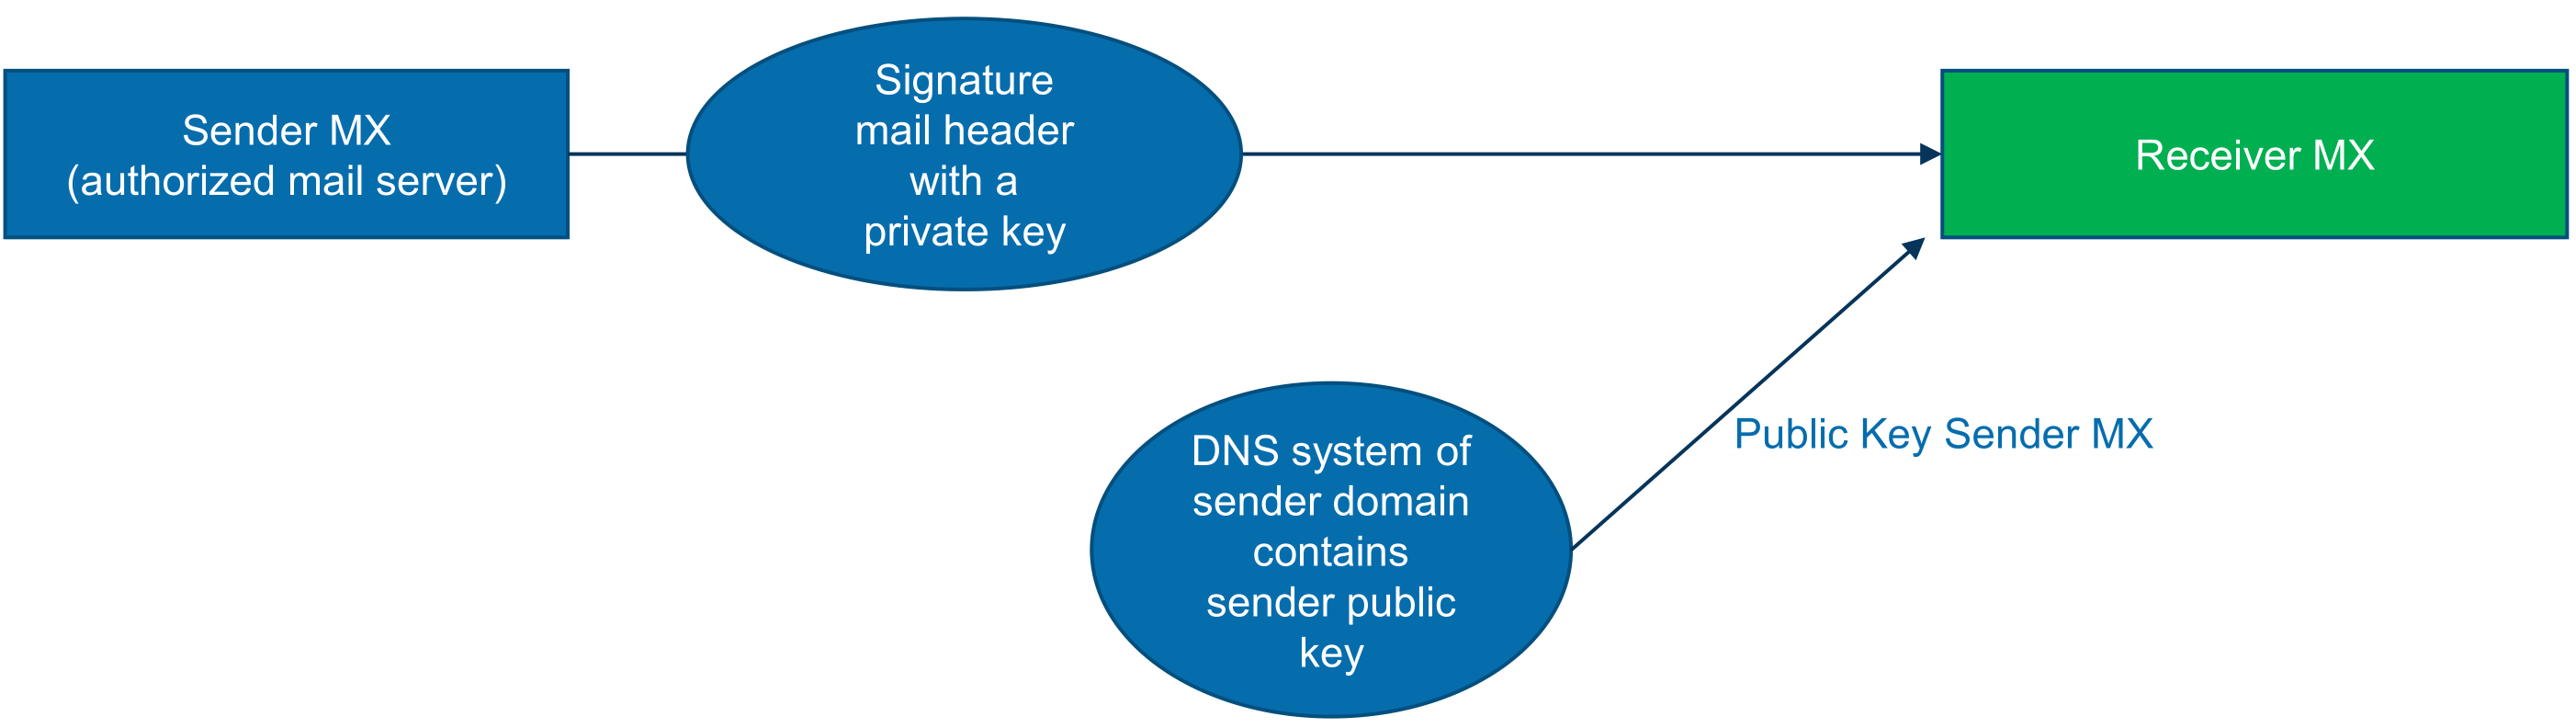
\includegraphics[width=\linewidth]{dkim-cryptography.png}\\

DKIM-Records are TXT DNS-Records. Used Codes in TXT content:
\begin{itemize}
  \item \textbf{v}: Version of record. E.g.: v=DKIM1
  \item \textbf{p}: Public Key
\end{itemize}

\subsubsection{How it works}
It works by adding a digital signature to the headers of an email message.
That signature can be validated against a public cryptographic key in the organization's Domain Name System (DNS) records. In general terms, the process works like this:\\

\begin{enumerate}
  \item A domain owner publishes a cryptographic public key as a specially-formatted TXT record in the domain's overall DNS records.
  \item When a mail message is sent by an outbound mail server, the server generates and attaches a unique DKIM signature header to the message.
  \item This header includes two cryptographic hashes, one of specified headers, and one of the message body (or part of it).
  \item The header contains information about how the signature was generated.
  \item When an inbound mail server receives an incoming email, it looks up the sender's public DKIM key in DNS.
  \item The inbound server uses this key to decrypt the signature and compare it against a freshly computed version.
  \item If the two values match, the message can be proved to authentic and unaltered in transit.
\end{enumerate}

\subsubsection{Check via console}
An DKIM check can be made via console.
Get the domain prefix from the header:\\
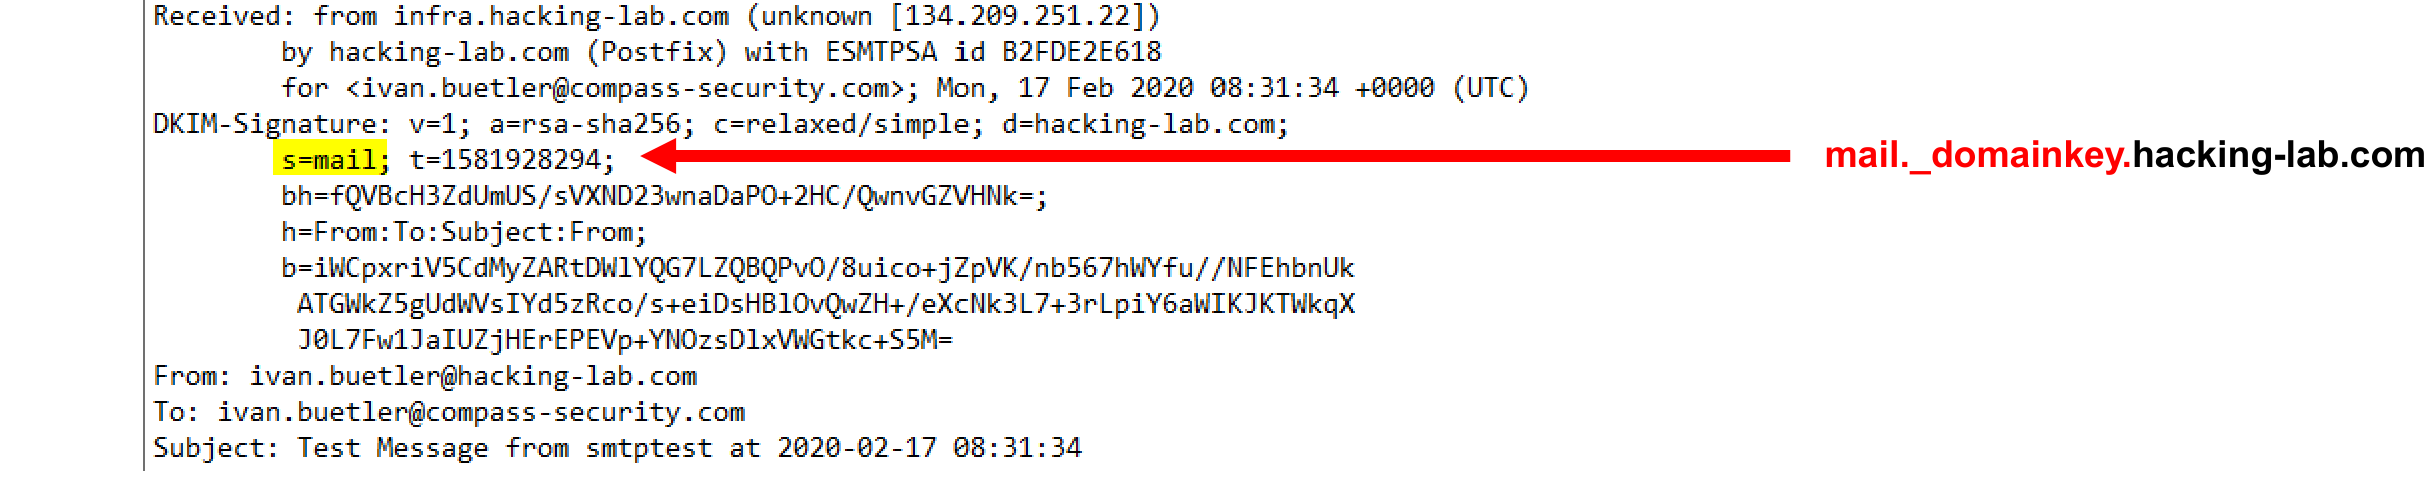
\includegraphics[width=\linewidth]{dkim-prefix-domain.png}

\begin{lstlisting}
  dig +short mail._domainkey.hacking-lab.com txt
  "v=DKIM1; k=rsa p=HGVZIUZVBUZM6mgVGV5TB8Mmvhg68Ngz66ZBFTBUGg7DDd"
\end{lstlisting}

\subsubsection{Where to check in metadata}
\paragraph{Passed}
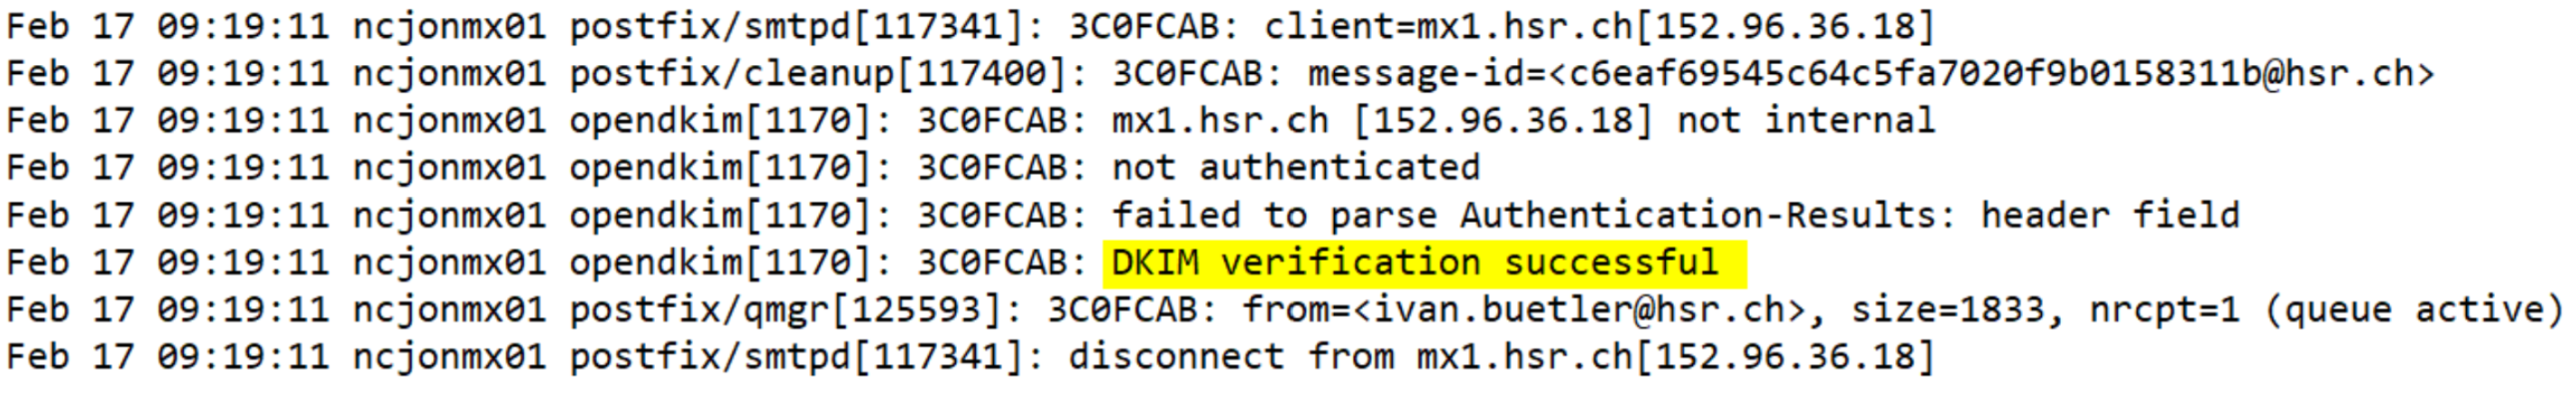
\includegraphics[width=\linewidth]{dkim-passed.png}

\paragraph{Failed}
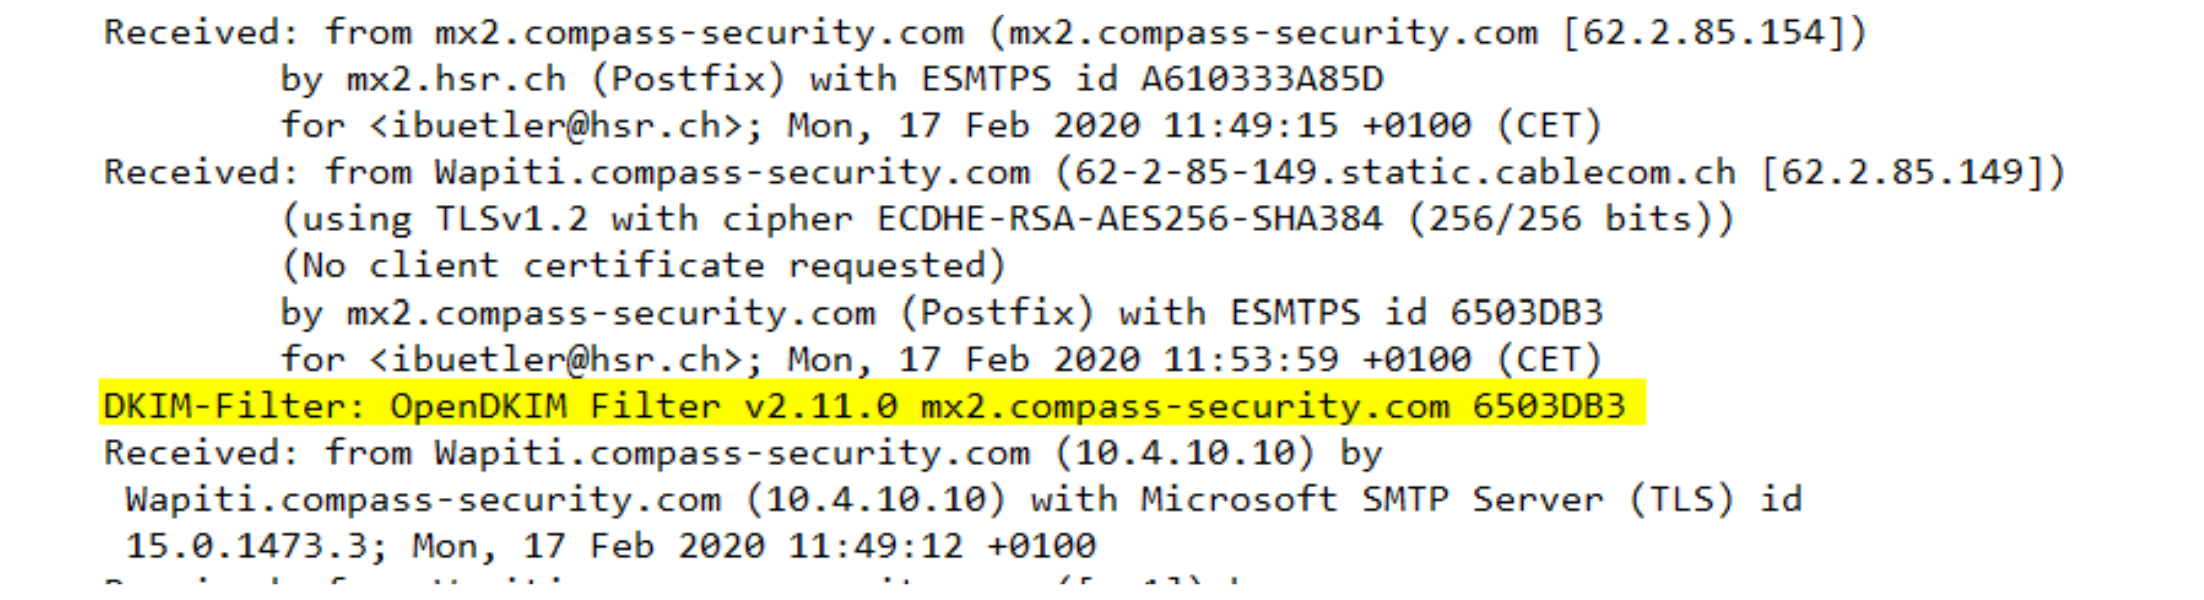
\includegraphics[width=\linewidth]{dkim-failed.png}




\subsection{DMARC}
Domain-based Message Authentication, Reporting, and Conformance.\\

DMARC unifies the SPF and DKIM authentication mechanisms into a common framework and allows domain owners to declare how they would like email from that domain to be handled if it fails an authorization test.\\

DKIM-Records are TXT DNS-Records. Used Codes in TXT content:
\begin{itemize}
  \item \textbf{v}: Version of record. E.g.: v=DMARC1
  \item \textbf{p}: Policy (e.g: none or quarantine)
  \item \textbf{rua}: (Report Email Address)
\end{itemize}

\subsubsection{Check via console}
An DMARK check can be made via console.
Get the domain prefix from the header:\\
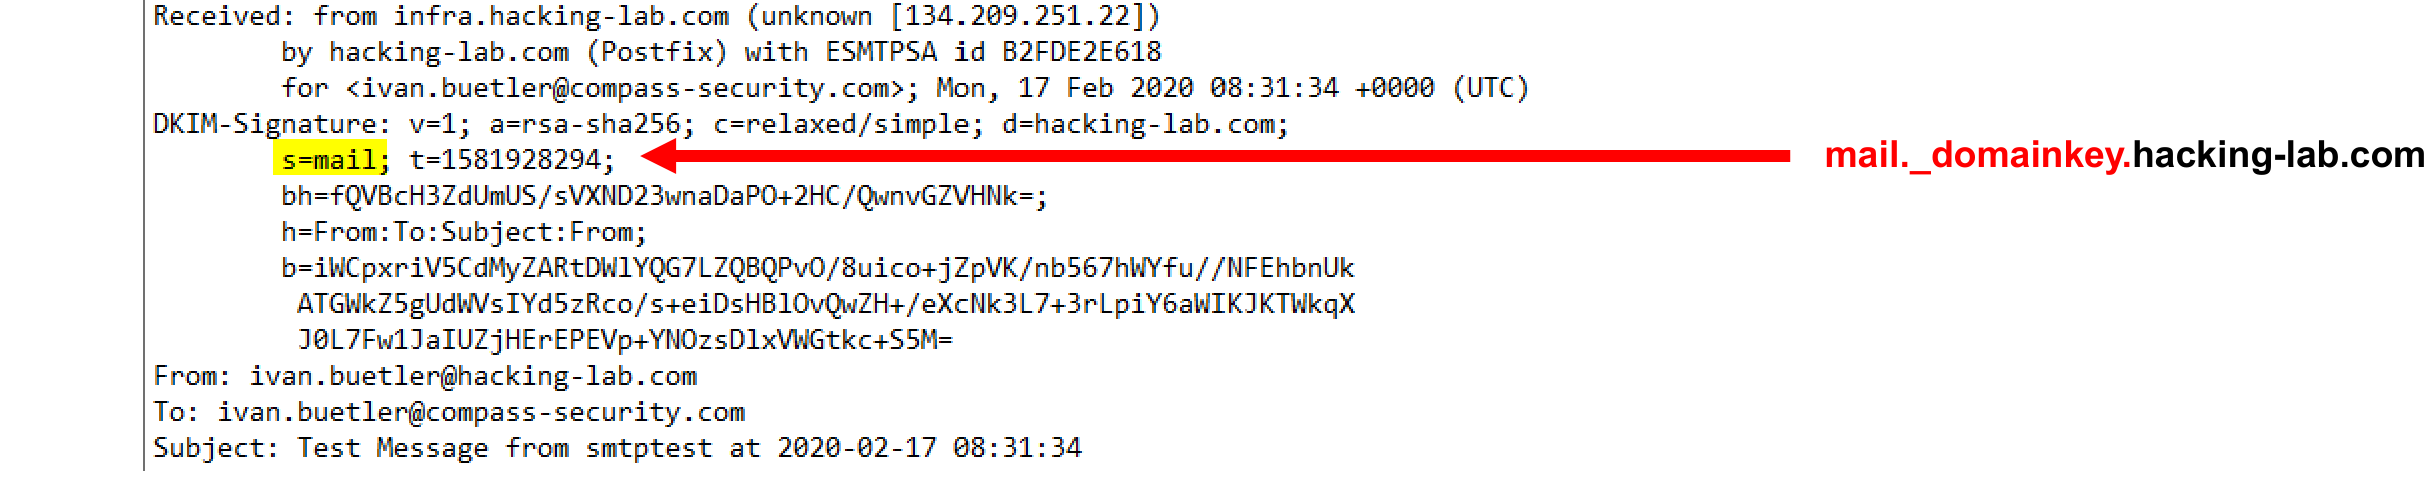
\includegraphics[width=\linewidth]{dkim-prefix-domain.png}

\begin{lstlisting}
  dig -t txt _dmarc.hacking-lab.com +short
  "v=DMARC1; p=none; rua=mailto:dmarc-reports-234324@hacking-lab.com; ri=86400"
\end{lstlisting}

\subsubsection{Where to check in metadata}
\paragraph{Passed}
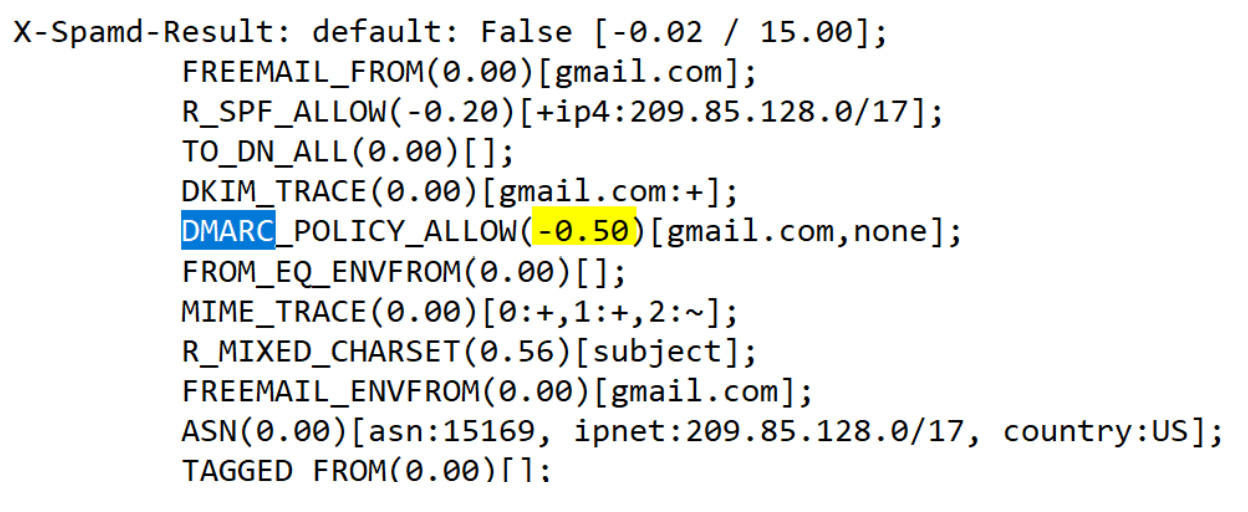
\includegraphics[width=\linewidth]{dmarc-passed.png}

\paragraph{Failed}
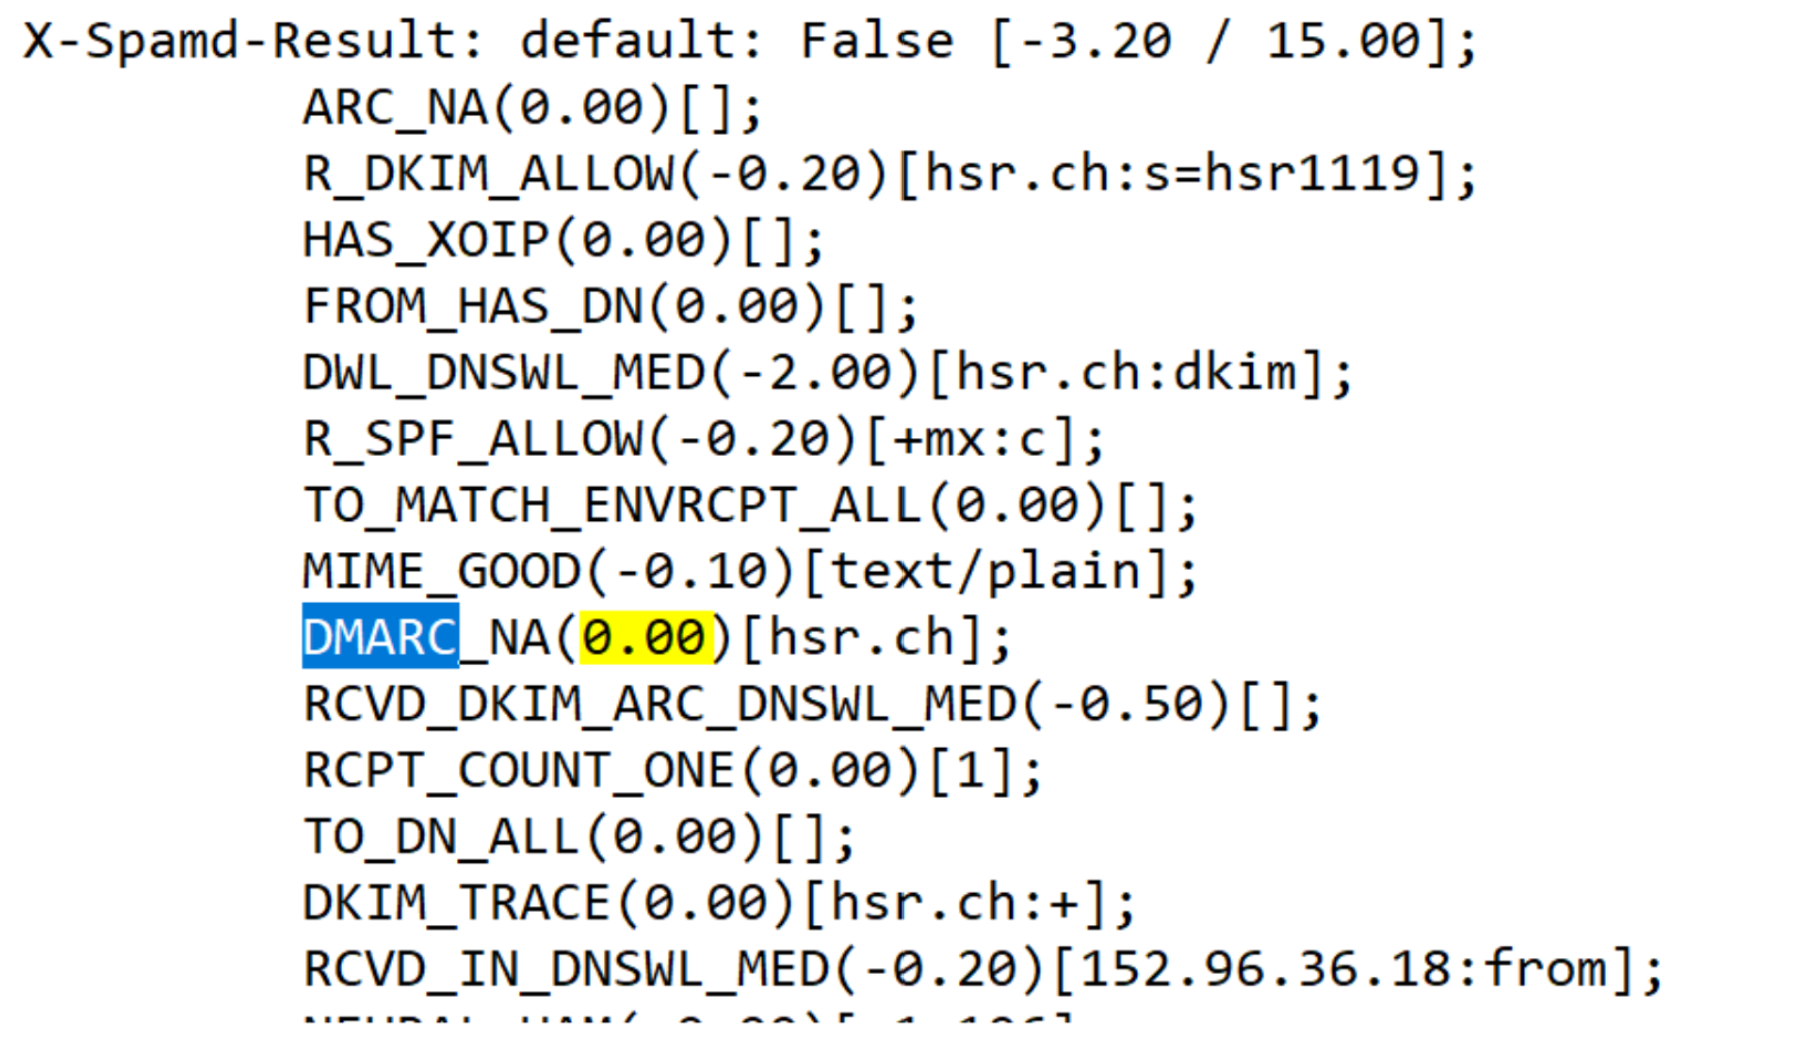
\includegraphics[width=\linewidth]{dmarc-failed.png}

\subsection{TLS Encryption}
\subsubsection{Where to check in metadata}
\paragraph{Passed}
\subparagraph{Example 1}
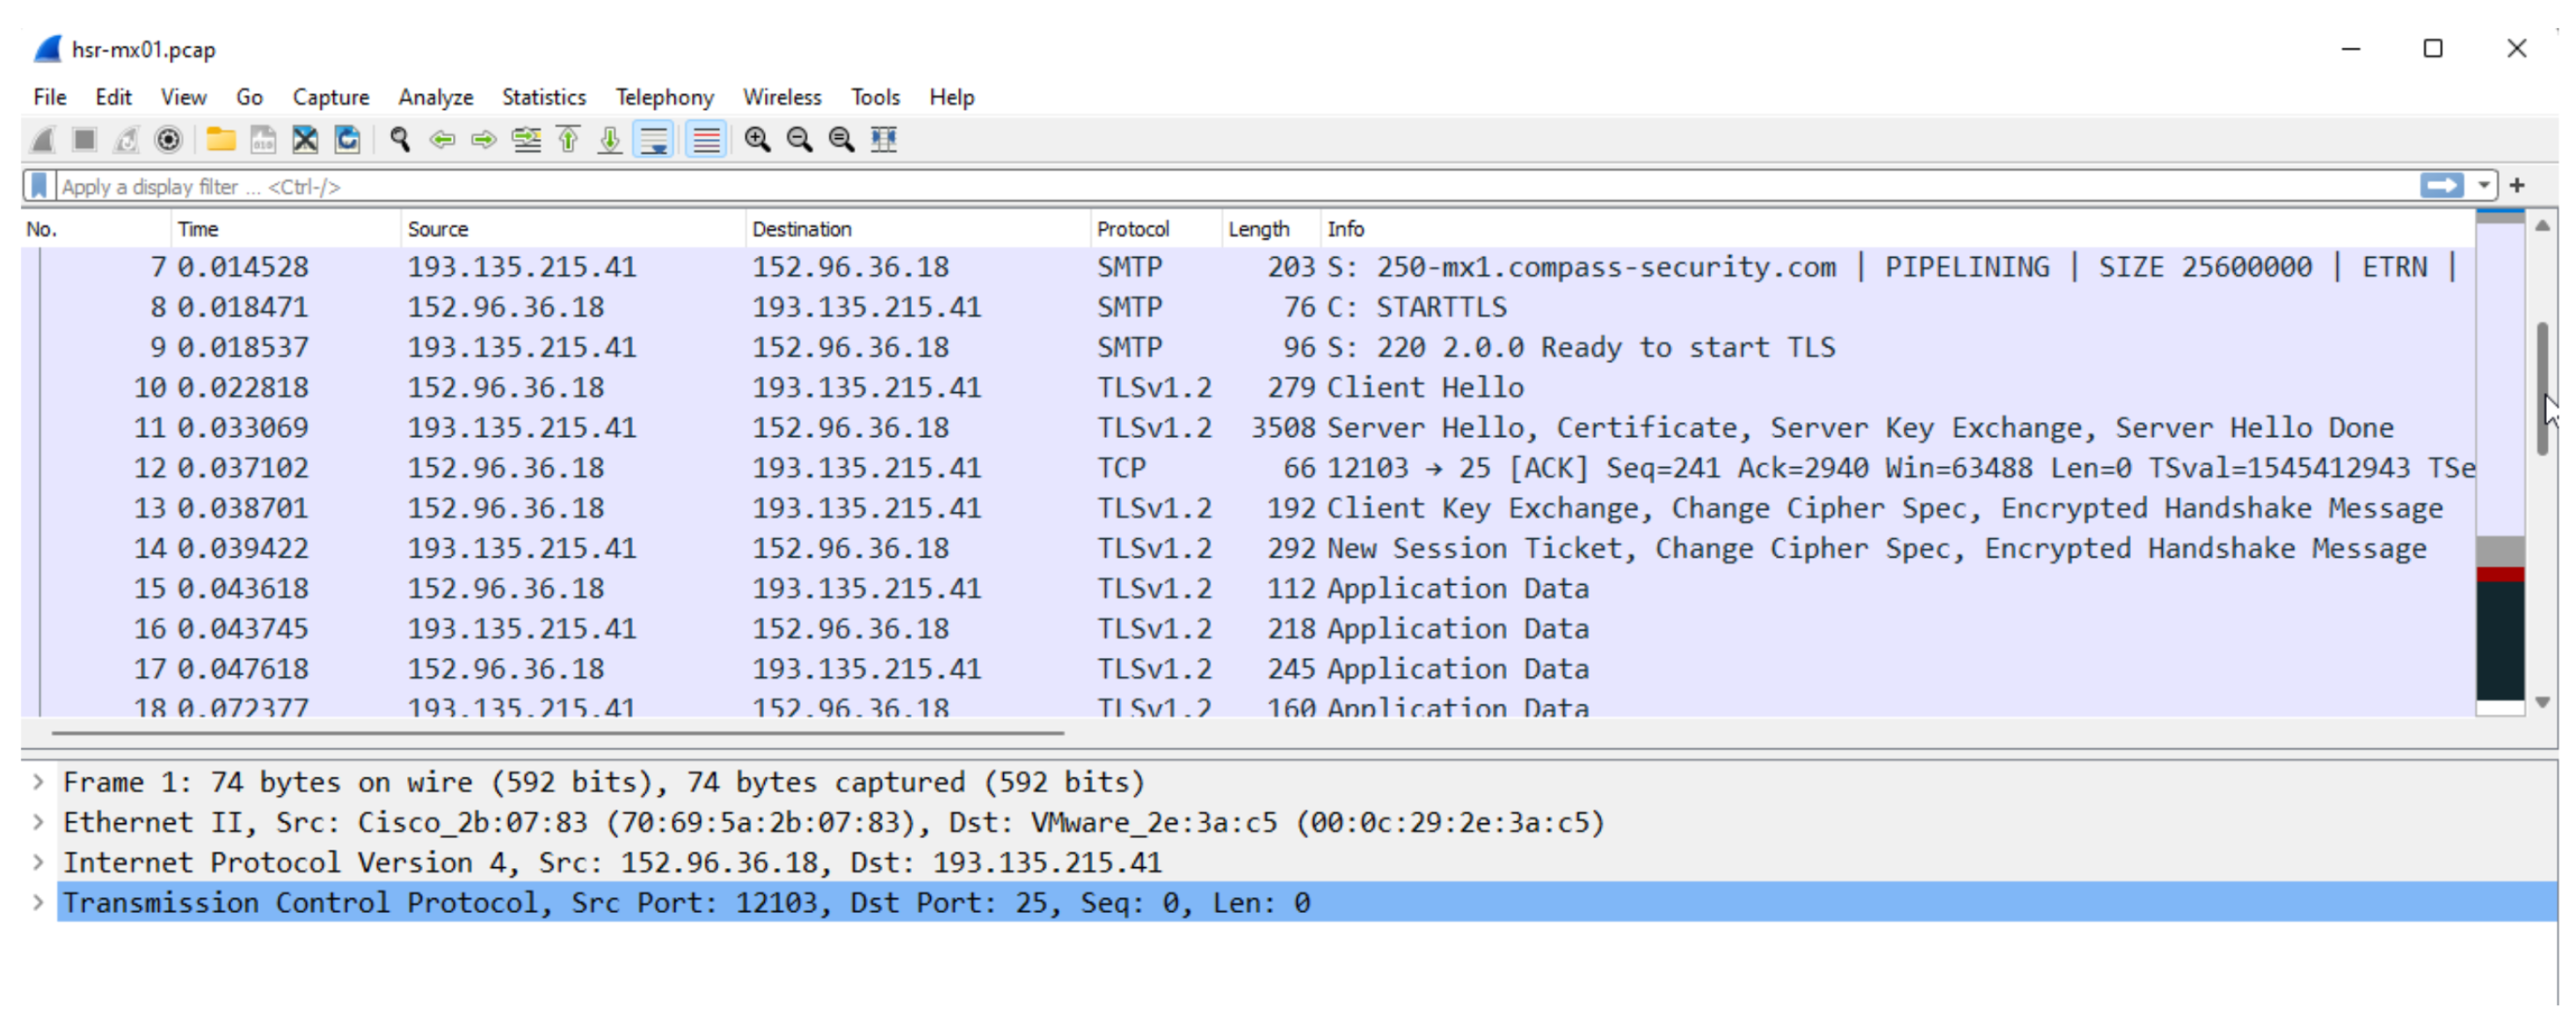
\includegraphics[width=\linewidth]{email-tls-passed-1.png}
\subparagraph{Example 2}
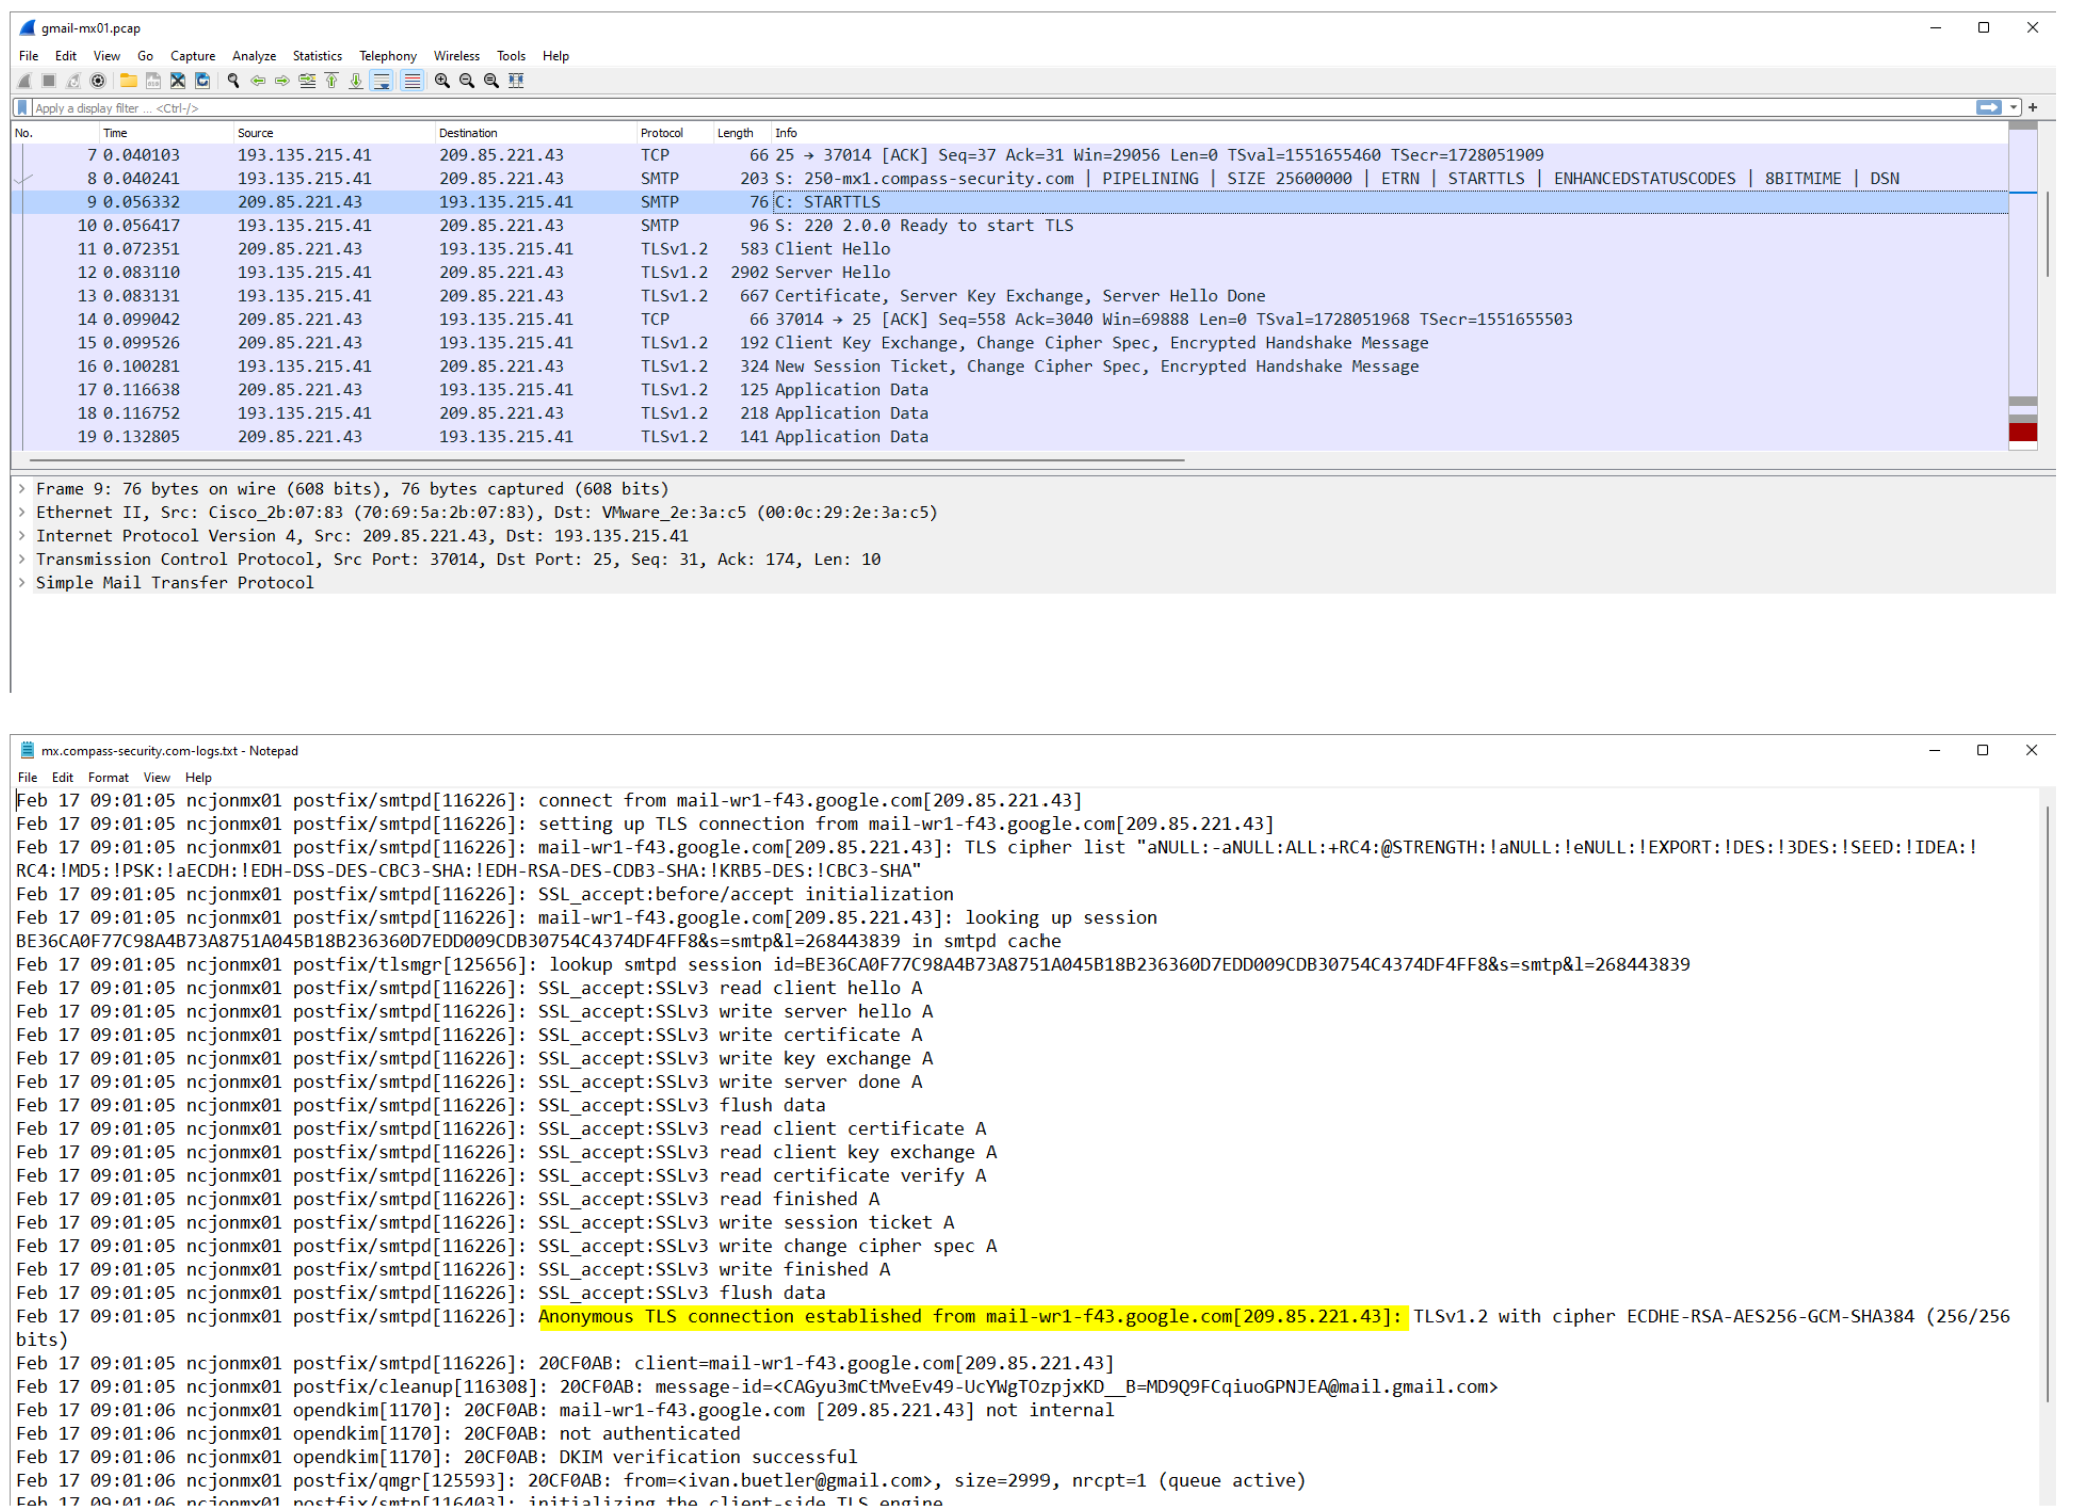
\includegraphics[width=\linewidth]{email-tls-passed-2.png}
\subparagraph{Example 3}
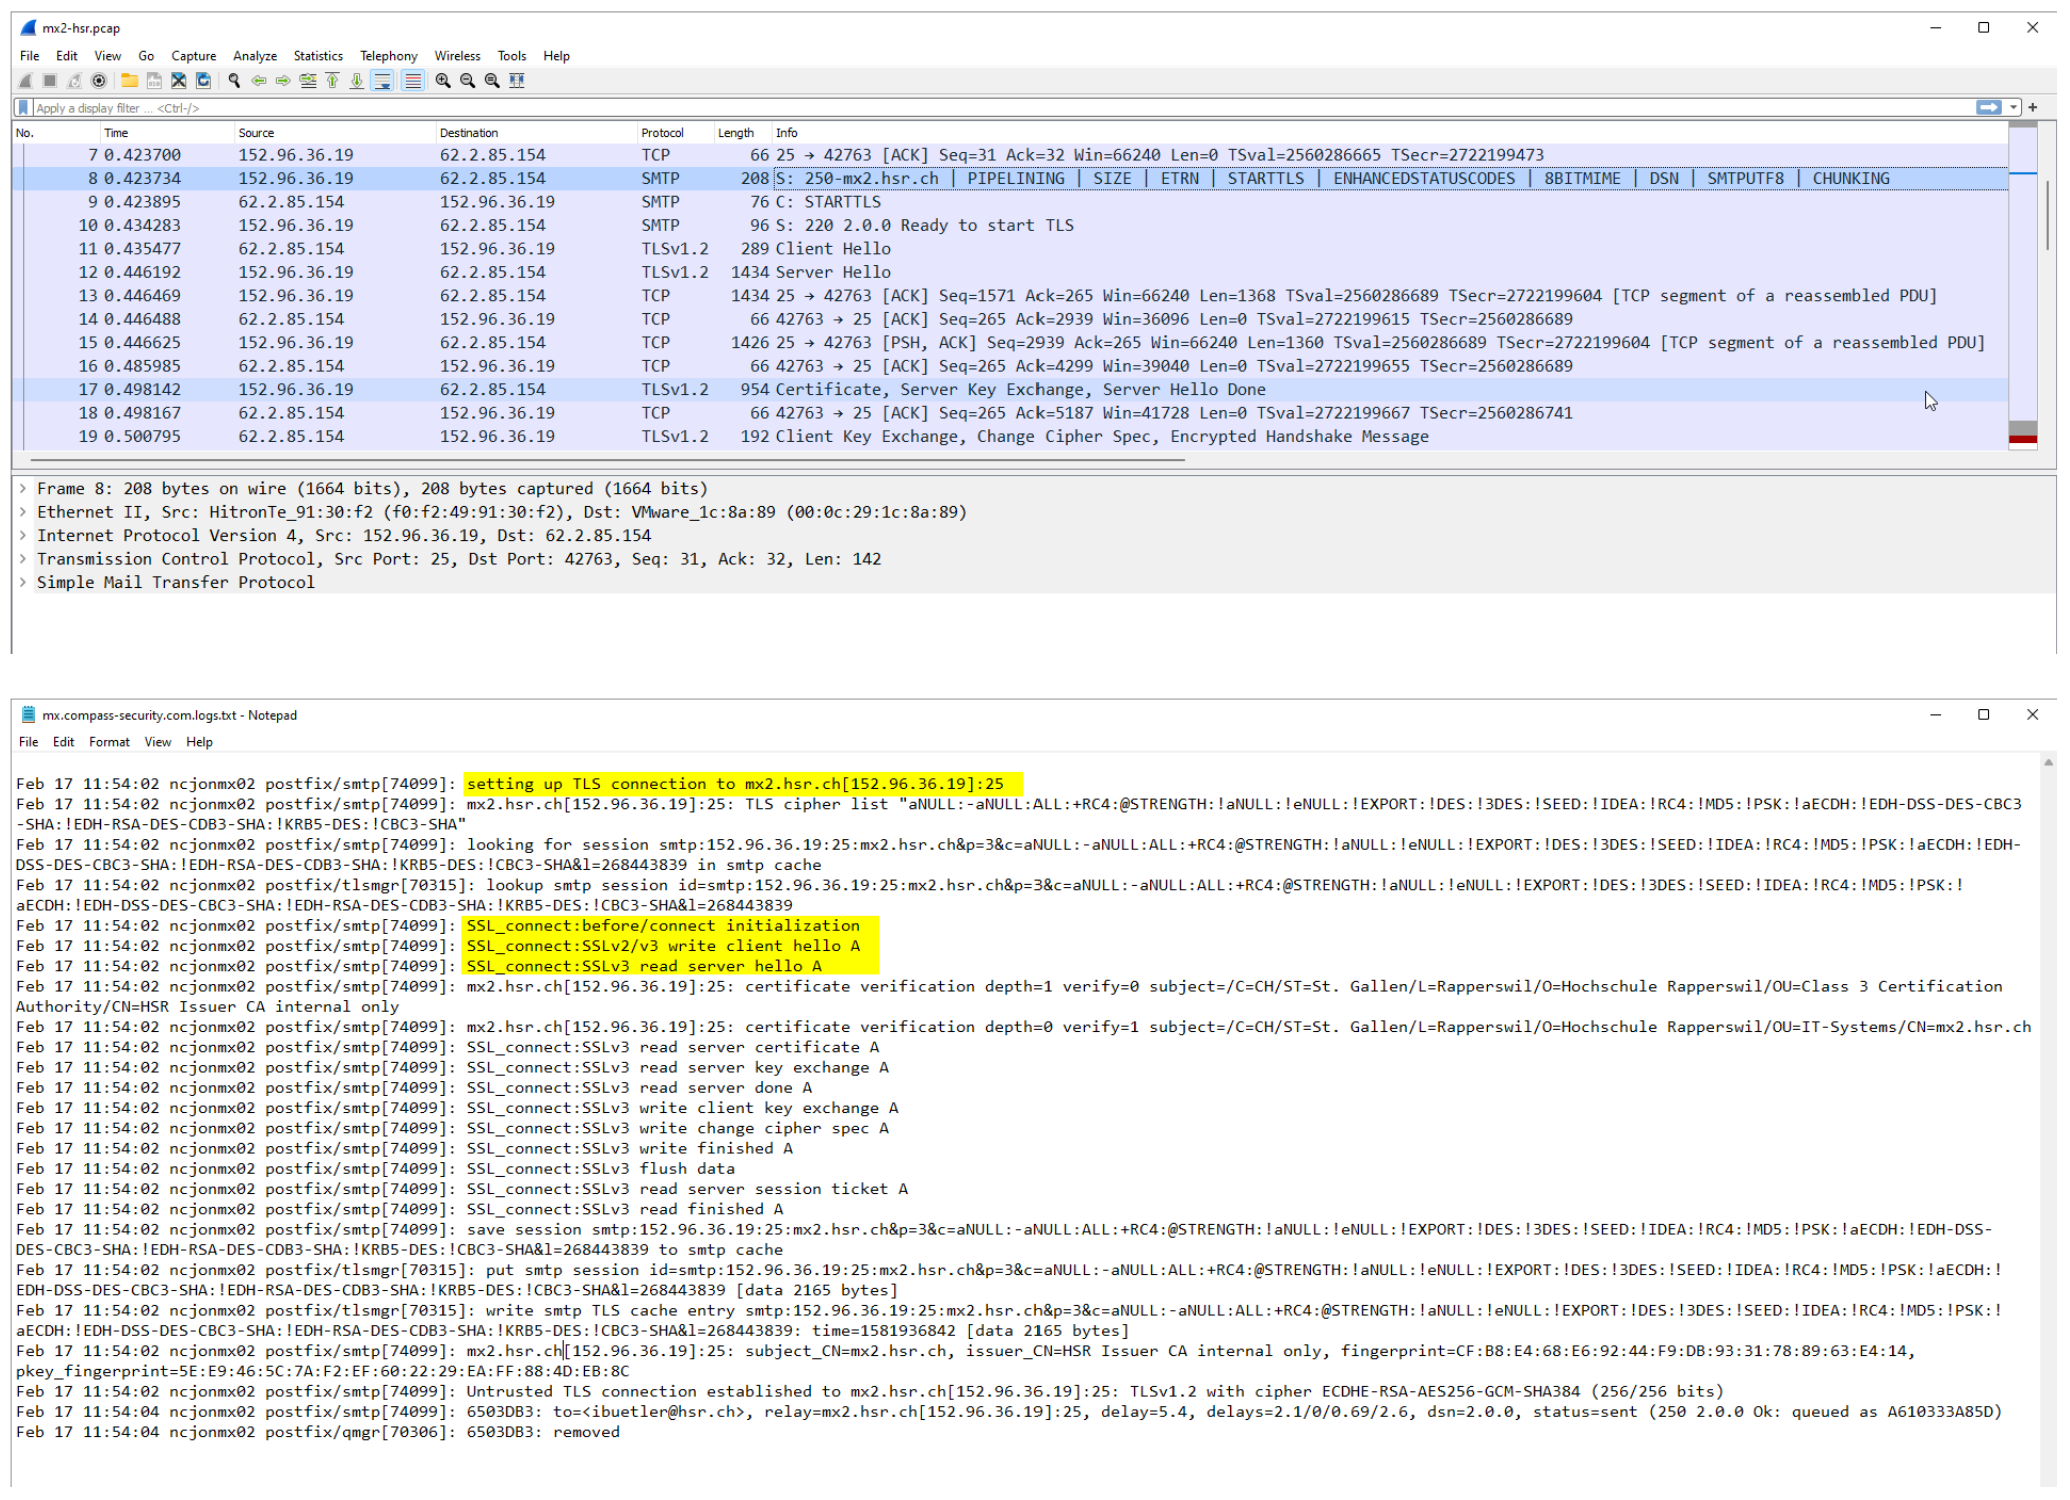
\includegraphics[width=\linewidth]{email-tls-passed-3.png}

\paragraph{Failed}
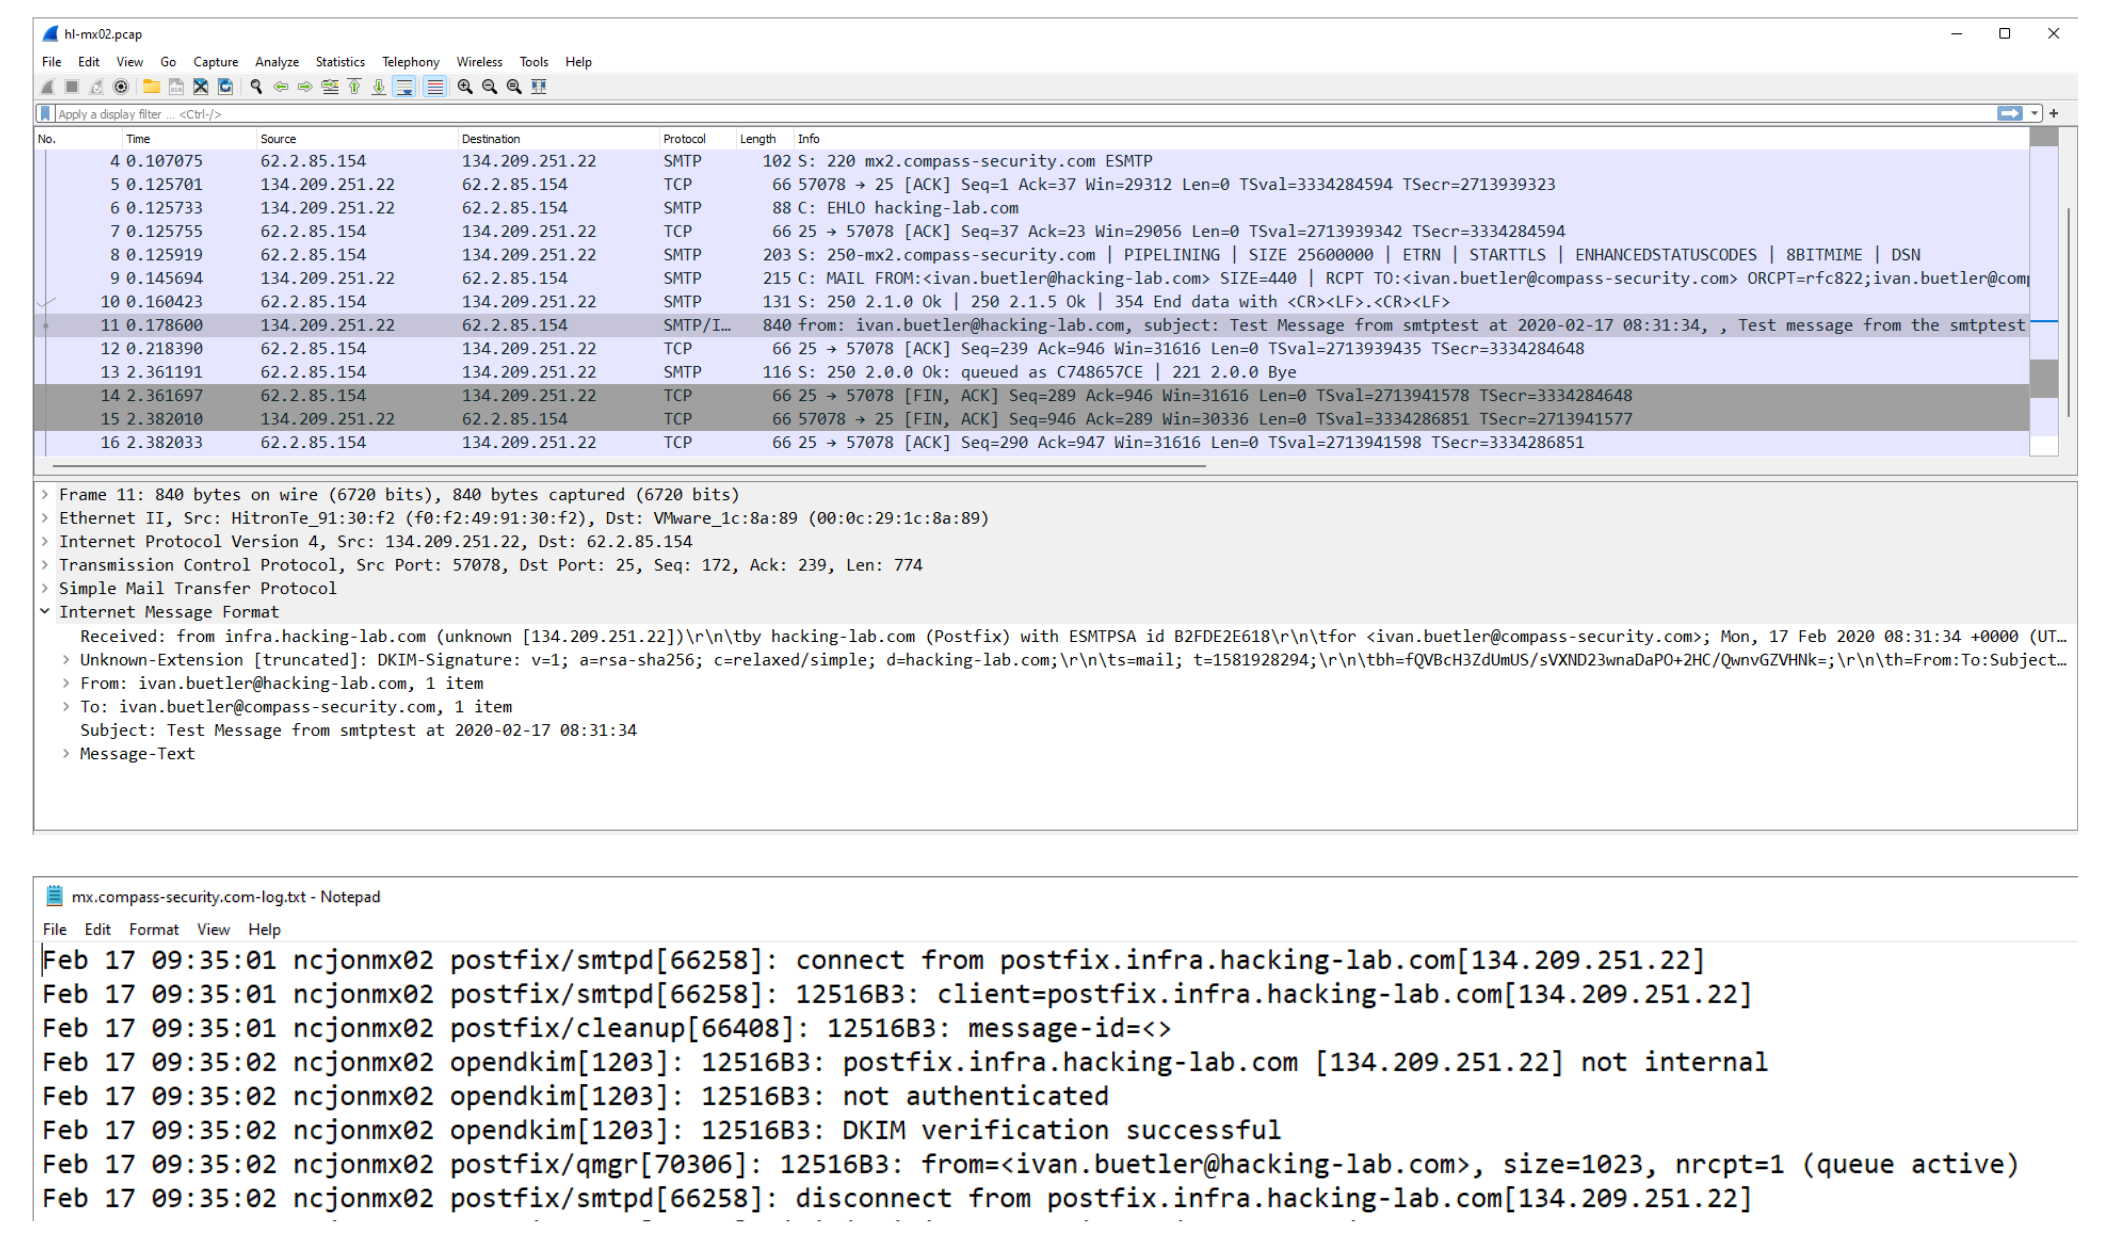
\includegraphics[width=\linewidth]{email-tls-failed.png}